% This is "sig-alternate.tex" V2.1 April 2013
% This file should be compiled with V2.5 of "sig-alternate.cls" May 2012
%
% This example file demonstrates the use of the 'sig-alternate.cls'
% V2.5 LaTeX2e document class file. It is for those submitting
% articles to ACM Conference Proceedings WHO DO NOT WISH TO
% STRICTLY ADHERE TO THE SIGS (PUBS-BOARD-ENDORSED) STYLE.
% The 'sig-alternate.cls' file will produce a similar-looking,
% albeit, 'tighter' paper resulting in, invariably, fewer pages.
%
% ----------------------------------------------------------------------------------------------------------------
% This .tex file (and associated .cls V2.5) produces:
%       1) The Permission Statement
%       2) The Conference (location) Info information
%       3) The Copyright Line with ACM data
%       4) NO page numbers
%
% as against the acm_proc_article-sp.cls file which
% DOES NOT produce 1) thru' 3) above.
%
% Using 'sig-alternate.cls' you have control, however, from within
% the source .tex file, over both the CopyrightYear
% (defaulted to 200X) and the ACM Copyright Data
% (defaulted to X-XXXXX-XX-X/XX/XX).
% e.g.
% \CopyrightYear{2007} will cause 2007 to appear in the copyright line.
% \crdata{0-12345-67-8/90/12} will cause 0-12345-67-8/90/12 to appear in the copyright line.
%
% ---------------------------------------------------------------------------------------------------------------
% This .tex source is an example which *does* use
% the .bib file (from which the .bbl file % is produced).
% REMEMBER HOWEVER: After having produced the .bbl file,
% and prior to final submission, you *NEED* to 'insert'
% your .bbl file into your source .tex file so as to provide
% ONE 'self-contained' source file.
%
% ================= IF YOU HAVE QUESTIONS =======================
% Questions regarding the SIGS styles, SIGS policies and
% procedures, Conferences etc. should be sent to
% Adrienne Griscti (griscti@acm.org)
%
% Technical questions _only_ to
% Gerald Murray (murray@hq.acm.org)
% ===============================================================
%
% For tracking purposes - this is V2.0 - May 2012

\documentclass{sig-alternate-05-2015}


\begin{document}

% Copyright
\setcopyright{acmcopyright}
%\setcopyright{acmlicensed}
%\setcopyright{rightsretained}
%\setcopyright{usgov}
%\setcopyright{usgovmixed}
%\setcopyright{cagov}
%\setcopyright{cagovmixed}


% DOI
\doi{10.475/123_4}

% ISBN
\isbn{123-4567-24-567/08/06}

%Conference
\conferenceinfo{EASE '17}{June 15--16, 2017, BTH - Karlskrona, Sweden}

\acmPrice{\$15.00}

%
% --- Author Metadata here ---
\conferenceinfo{EASE}{'17 BTH - Karlskrona, Sweden}
%\CopyrightYear{2007} % Allows default copyright year (20XX) to be over-ridden - IF NEED BE.
%\crdata{0-12345-67-8/90/01}  % Allows default copyright data (0-89791-88-6/97/05) to be over-ridden - IF NEED BE.
% --- End of Author Metadata ---

\title{Seeking for the formalization of Experimentation in Software Engineering: An Empirical Study\titlenote{}}
%\subtitle{[Extended Abstract]
%\titlenote{A full version of this paper is available as
%\textit{Author's Guide to Preparing ACM SIG Proceedings Using
%\LaTeX$2_\epsilon$\ and BibTeX} at
%\texttt{www.acm.org/eaddress.htm}}}
%
% You need the command \numberofauthors to handle the 'placement
% and alignment' of the authors beneath the title.
%
% For aesthetic reasons, we recommend 'three authors at a time'
% i.e. three 'name/affiliation blocks' be placed beneath the title.
%
% NOTE: You are NOT restricted in how many 'rows' of
% "name/affiliations" may appear. We just ask that you restrict
% the number of 'columns' to three.
%
% Because of the available 'opening page real-estate'
% we ask you to refrain from putting more than six authors
% (two rows with three columns) beneath the article title.
% More than six makes the first-page appear very cluttered indeed.
%
% Use the \alignauthor commands to handle the names
% and affiliations for an 'aesthetic maximum' of six authors.
% Add names, affiliations, addresses for
% the seventh etc. author(s) as the argument for the
% \additionalauthors command.
% These 'additional authors' will be output/set for you
% without further effort on your part as the last section in
% the body of your article BEFORE References or any Appendices.

\numberofauthors{3} %  in this sample file, there are a *total*
% of EIGHT authors. SIX appear on the 'first-page' (for formatting
% reasons) and the remaining two appear in the \additionalauthors section.
%
\author{
% You can go ahead and credit any number of authors here,
% e.g. one 'row of three' or two rows (consisting of one row of three
% and a second row of one, two or three).
%
% The command \alignauthor (no curly braces needed) should
% precede each author name, affiliation/snail-mail address and
% e-mail address. Additionally, tag each line of
% affiliation/address with \affaddr, and tag the
% e-mail address with \email.
%
% 1st. author
\alignauthor
Efra�n R. Fonseca C.\\
       \affaddr{Universidad de las Fuerzas Armadas ESPE}\\
       \affaddr{Avda. General Rumi�ahui s/n}\\
       \affaddr{Sangolqu�, Ecuador}\\
       \email{erfonseca@espe.edu.ec}
% 2nd. author
\alignauthor
Oscar Dieste\\
       \affaddr{Universidad Polit\'ecnica de Madrid}\\
       \affaddr{Boadilla del Monte, 28660}\\
       \affaddr{Madrid, Spain}\\
       \email{odieste@fi.upm.es}
% 3rd. author
%\alignauthor Alejandra Ponce\\
%       \affaddr{Universidad de las Fuerzas Armadas ESPE}\\
%       \affaddr{Avda. General Rumi�ahui s/n}\\
%       \affaddr{Sangolqu�, Ecuador}\\
%       \email{adponce@espe.edu.ec}
%\and  % use '\and' if you need 'another row' of author names
% 4th. author
\alignauthor Mar�a Emilia Medina\\
       \affaddr{Universidad de las Fuerzas Armadas ESPE}\\
       \affaddr{Avda. General Rumi�ahui s/n}\\
       \affaddr{Sangolqu�, Ecuador}\\
       \email{memedina@espe.edu.ec}
% 5th. author
%\alignauthor Geovanny Raura\\
%       \affaddr{Universidad de las Fuerzas Armadas ESPE}\\
%       \affaddr{Avda. General Rumi�ahui s/n}\\
%       \affaddr{Sangolqu�, Ecuador}\\
%       \email{jgraura@espe.edu.ec}
% 6th. author
\and
\alignauthor Natalia Juristo\\
       \affaddr{Universidad Polit\'ecnica de Madrid}\\
       \affaddr{Boadilla del Monte, 28660}\\
       \affaddr{Madrid, Spain}\\
       \email{natalia@fi.upm.es}\\
       \affaddr{~}\\
       \affaddr{University of Oulu}\\
       \affaddr{Oulu, Finland}\\
       \email{natalia.juristo@oulu.fi}
}
% There's nothing stopping you putting the seventh, eighth, etc.
% author on the opening page (as the 'third row') but we ask,
% for aesthetic reasons that you place these 'additional authors'
% in the \additional authors block, viz.
%\additionalauthors{Additional authors: John Smith (The Th{\o}rv{\"a}ld Group,
%email: {\texttt{jsmith@affiliation.org}}) and Julius P.~Kumquat
%(The Kumquat Consortium, email: {\texttt{jpkumquat@consortium.net}}).}
%\date{30 July 1999}
% Just remember to make sure that the TOTAL number of authors
% is the number that will appear on the first page PLUS the
% number that will appear in the \additionalauthors section.
\maketitle

\begin{abstract}
\textbf{\textendash\textendash \textit{Background: }}Several decades have passed since the first experiment was carried out in software engineering (SE). Since then, the number of experiments undertaken in academy and lately in industry have had a significant upturn. However, some SE researchers consider that there is still uncertainty about what activities have to be performed before, during and after an experiment. \textbf{\textit{Aim: }}To identify and validate constraints surrounding the experimentation in SE, on the basis of the formality signs identified within the experimental process of tradicional disciplines. \textbf{\textit{Method: }}An exploratory study based on empirical mix methods was conducted, which involved the identification of activities complexity in practice regarding the experimentation in SE; learning about the experimental process performed in a traditional discipline to identify particular constraints within experimentation in SE through comparison; and the validation of experimental SE constraints within empirical software engineering community. \textbf{\textit{Results: }}Conceptual and process models obtained around the observation and the participation of the SE experimental activities and other traditional discipline, respectively, made it possible to identify some constraints within the SE experimental process through comparison, which was validated by the ESE community. \textbf{\textit{Conclusions: }}There are activities and concepts used in the experimental process of traditional disciplines that could be applied in the experimental SE in order to improve its process, which is claimed by the ESE community.
\end{abstract}
%\textbf{\textendash\textendash \textit{Antecedentes: }}Han pasado varias d�cadas desde que se llev� a cabo el primer experimento en Ingenier�a de Software (SE). Desde entonces, ha habido un importante repunte en el n�mero de experimentos realizados en la academia y �ltimamente en la industria. No obstante, algunos investigadores en SE consideran que a�n existe incertidumbre respecto a las actividades a realizar antes, durante y despu�s de un experimento. \textbf{\textit{Objetivo: }}Identificar y validar la problem�tica en torno a la Experimentaci�n en SE, tomando como referencia los indicios de formalidad identificados en el proceso de experimentaci�n de las disciplinas tradicionales. \textbf{\textit{Metodolog�a: }}Se realiz� un estudio exploratorio basado en m�todos emp�ricos mixtos para: (1) indagar sobre la problem�tica en torno a la experimentaci�n en SE dentro de un grupo de investigaci�n representativo en la comunidad de SE emp�rica (ESE), (2) aprender del proceso de experimentaci�n en una disciplina tradicional e identificar la problem�tica particular de la Experimentaci�n en SE, y (3) validar la generalidad de la problem�tica identificada en la experimentaci�n en SE. \textbf{\textit{Resultados: }}Se obtuvieron modelos conceptuales y de proceso que permitieron entender de forma expl�cita la experimentaci�n llevada a cabo en la SE, as� como sus carencias respecto a una disciplina experimental tradicional y finalmente se comprob� que las carencias identificadas en la SE son generales. \textbf{\textit{Conclusiones: }} Existen actividades y conceptos utilizados en el proceso de experimentaci�n de las disciplinas tradicionales que son semejantes a los utilizados en el proceso de experimentaci�n es SE. Sin embargo, existen actividades y conceptos que podr�an ser aplicados en la SE para mejorar su proceso de experimentaci�n.

% The code below should be generated by the tool at
% http://dl.acm.org/ccs.cfm
% Please copy and paste the code instead of the example below. 
%
\begin{CCSXML}
<ccs2012>
 <concept>
  <concept_id>10010520.10010553.10010562</concept_id>
  <concept_desc>Computer systems organization~Embedded systems</concept_desc>
  <concept_significance>500</concept_significance>
 </concept>
 <concept>
  <concept_id>10010520.10010575.10010755</concept_id>
  <concept_desc>Computer systems organization~Redundancy</concept_desc>
  <concept_significance>300</concept_significance>
 </concept>
 <concept>
  <concept_id>10010520.10010553.10010554</concept_id>
  <concept_desc>Computer systems organization~Robotics</concept_desc>
  <concept_significance>100</concept_significance>
 </concept>
 <concept>
  <concept_id>10003033.10003083.10003095</concept_id>
  <concept_desc>Networks~Network reliability</concept_desc>
  <concept_significance>100</concept_significance>
 </concept>
</ccs2012>  
\end{CCSXML}

\ccsdesc[500]{Computer systems organization~Embedded systems}
\ccsdesc[300]{Computer systems organization~Redundancy}
\ccsdesc{Computer systems organization~Robotics}
\ccsdesc[100]{Networks~Network reliability}


%
% End generated code
%

%
%  Use this command to print the description
%
\printccsdesc

% We no longer use \terms command
%\terms{Theory}

\keywords{Software Engineering, Empirical Software Engineering, Experimentation in Software Engineering, Case Study}

\section{Introduction}\label{sec-introduction}
SE researchers have started to perform introspection on how empirical Software Engineering (SE) functions, as it had happened in other traditional disciplines, such as Medicine \cite{altman-1998-statistical-reviewing-medical}. As Kitchenham et al. \cite{Kitchenham2002-GuideLinesESE} point it out: \textquotedblleft If researchers have difficulty in a discipline such as medicine, which has a rich history of empirical research, it is hardly surprising that software engineering researchers have problems\textquotedblright.

Los pocos estudios existentes han abordado principalmente aspectos estad�sticos. Por ejemplo, Vegas et al. \cite{Vegas-2016-Crossover-Designs-ESE} han estudiado en qu� medida los dise�os cross-over son correctamente analizados. Del mismo modo, \rodrinote{[COMPLETAR DE ACUERDO AL PAPER DE ROLANDO]} Desde una perspectiva m�s general, Reyes et al. \cite{Reyes-2018-Statistical-Errors-in-SE} han determinado emp�ricamente la existencia de distintos tipos de errores en experimentos de SE. J{\o}rgensen et al. \cite{Jorgensen-2016-Incorrects-Results-SEE} llegan a afirmar que una gran parte de los resultados experimentales en SE son falsos.

 This issue is not privative of SE. Other experimental disciplines, such as Biotechnology \cite{Kumar-2014-design-experiment-bioprocessing}, Medicine and Psychology, reported similar problems at some point \cite{Garcia-2012-Cienci-Abierta}. \rodrinote{[ESTE P�RRAFO DEBEB SER CAMBIADO DE ACUERDO AL PAPER DE ROLANDO]}
 
 Sin embargo, los aspectos matem�ticos

We performed a mix-methods empirical study to inquire the current state of the experimentation process' formalization into SE, compared with the traditional experimental disciplines. Firstly, we carried out a comparative observational study about the experimentation process that takes place in SE and a traditional experimental discipline, such as Biotechnology. Some representative research groups of both communities were studied to give validity to this study. However, we surveyed the most representative researchers of the ESE community in order to validate and generalize the findings obtained in the first study.

The results o this study contribute to SE research through the identification of experiment activities in another traditional discipline, which could enhance the formalization of experiment process in specific research areas of SE. We believe that such formalization is possible if the harmony of experiment tasks are achieved through particular protocols per research area. \rodrinote{\textquotedblleft COMPLETAR\textquotedblright}.

The remainder of the paper is organized as follows: Section \ref{sec-background} introduces the context which motivated the research. Research methodology is described in Section \ref{sec-methology}. Section \ref{sec-ESE-etnography} shows the results of the ethnographic study carried out in a representative SE research group. Afterward, Section \ref{sec-survey} details the results of the validation about SE experimentation issues identified. Section \ref{sec-bio-etnography} specifies the ethnographic study performed in specific Biotechnology areas. A summarized discussion about threats to validity identified is presented in Section \ref{sec-threats}. Finally, the discussion and main conclusions are presented in Section \ref{sec-discussion-conclusions}.
\rodrinote{OSCAR POR FAVOR REVISA NUEVAMENTE LA INTRODUCCI�N}.

\section{Background}\label{sec-background}
Desde sus inicios la experimentaci�n en SE ha pretendido consolidarse a trav�s de propuestas metodol�gicas que gu�en su proceso \cite{Basili-1986-ESE,Juristo2001,Kitchenham2002-GuideLinesESE,Wohlin2000}, las replicaciones \cite{Solari2006-ClasAnalLabPaq} e incluso sus reportes \cite{Jedlitschka2005-GuideLinesESE,Carver2010-GuidelinesReplication,Kitchenham:2008b}; de hecho, las instancias de experimentos se han incrementado notablemente en los �ltimos tiempos \cite{Sjoberg2005-surveyexperimentsESE,Zendler2001,Dieste2011-CompAnalMetaWhenWich}, a su vez la importancia de sus hallazgos e indica que este paradigma est� bien posicionado en SE.

No obstante, en la pr�ctica se aplican una diversidad de protocolos y formatos de reporte que superan abismalmente las propuestas formales antes mencionadas. Esta condici�n da indicios para asumir que cada experimento en SE incluye actividades diversas que han sido adoptadas de acuerdo a la concepci�n particular de cada investigador o grupo de investigadores y causa incertidumbre en torno al efecto que esto podr�a implicar. En la literatura se han publicado diversos estudios que sugieren circunstancias que podr�an corroboran esta situaci�n, de los cuales a continuaci�n se citan algunos ejemplos.

Magalh�es et al. \cite{Demagalhaes-2015-SMS-Replications} indican que \textquotedblleft Replications of empirical studies play important roles in the construction of knowledge\textquotedblright. No obstante, en el mismo estudio se menciona que las replicaciones en SE son muy complejas de realizar, debido probablemente (entre otras causas) a las casi inevitables variaciones que existen entre el estudio original y la replicaci�n por razones intencionadas o no intencionadas. Consecuentemente, no existe armon�a entre el creciente n�mero de experimentos en SE y el n�mero de replicaciones existentes \cite{da-silva-2012-replication-on-empirical-studies}. 


 

Por el contrario, otras disciplinas experimentales tradicionales tienen currently a very rigorous and uniform process \cite{stoker-2009-iLAP-bioinformatics,Jones-2007-FUGE,ko-2012-SMISB}. No obstante, los investigadores en SE han iniciando la realizaci�n de una introspecci�n en su disciplina encontrando de la SE es una disciplina candidata a que en sus instancias experimentales se encuentren errores

\section{Methodology}\label{sec-methology}
\subsection{Research objectives}
El objetivo de esta investigaci�n se muestra en la tabla \ref{tbl:objetivo-GQM} en formato  Goal Question Metric (GQM) \cite{Basili-1992-SwModMeasGQM}.

\begin{table}[htb]
\centering
\caption{Objetivo de Investigaci�n en Formato GQM}
\label{tbl:objetivo-GQM}
\begin{tabular}{|r|p{3.5cm}|}
\hline
\textbf{Estudiar:} & las actividades llevadas a cabo en la SE, para la planificaci�n, dise�o, ejecuci�n, an�lisis y reporte de experimentos\\
\hline
\textbf{con el prop�sito de:} & identificar problemas y debilidades en la pr�ctica experimental\\
\hline
\textbf{con respecto a:} & las actividades realizadas en otras disciplinas experimentales asentadas\\
\hline
\textbf{desde el punto de vista del:} & investigador\\
\hline
\textbf{en el contexto de:} & la investigaci�n experimental.\\
\hline
\end{tabular}
\end{table}

\subsection{Research design}
A mixed research methodology was applied, which is divided into 3 stages, as shown in the Figure \ref{fig-research-methodology}. First, we conducted an ethnographical study to observe how a representative SE research group functions. Since the results obtained from a unique research group are not necessarily generalizable to the entire ESE community, we conducted a survey in order to asses wether our findings could be extrapolated to the entire ESE community. Finally, a second ethnographical study was carried out in another research group. This research group was not related to SE, but to Bioengineering. This second group, in some way, acted as a control group. The aim of this second ethnography was to highlight those SE practices that differed strongly from those of another more traditional, and well-established  discipline.

\begin{figure*}
	\centering
	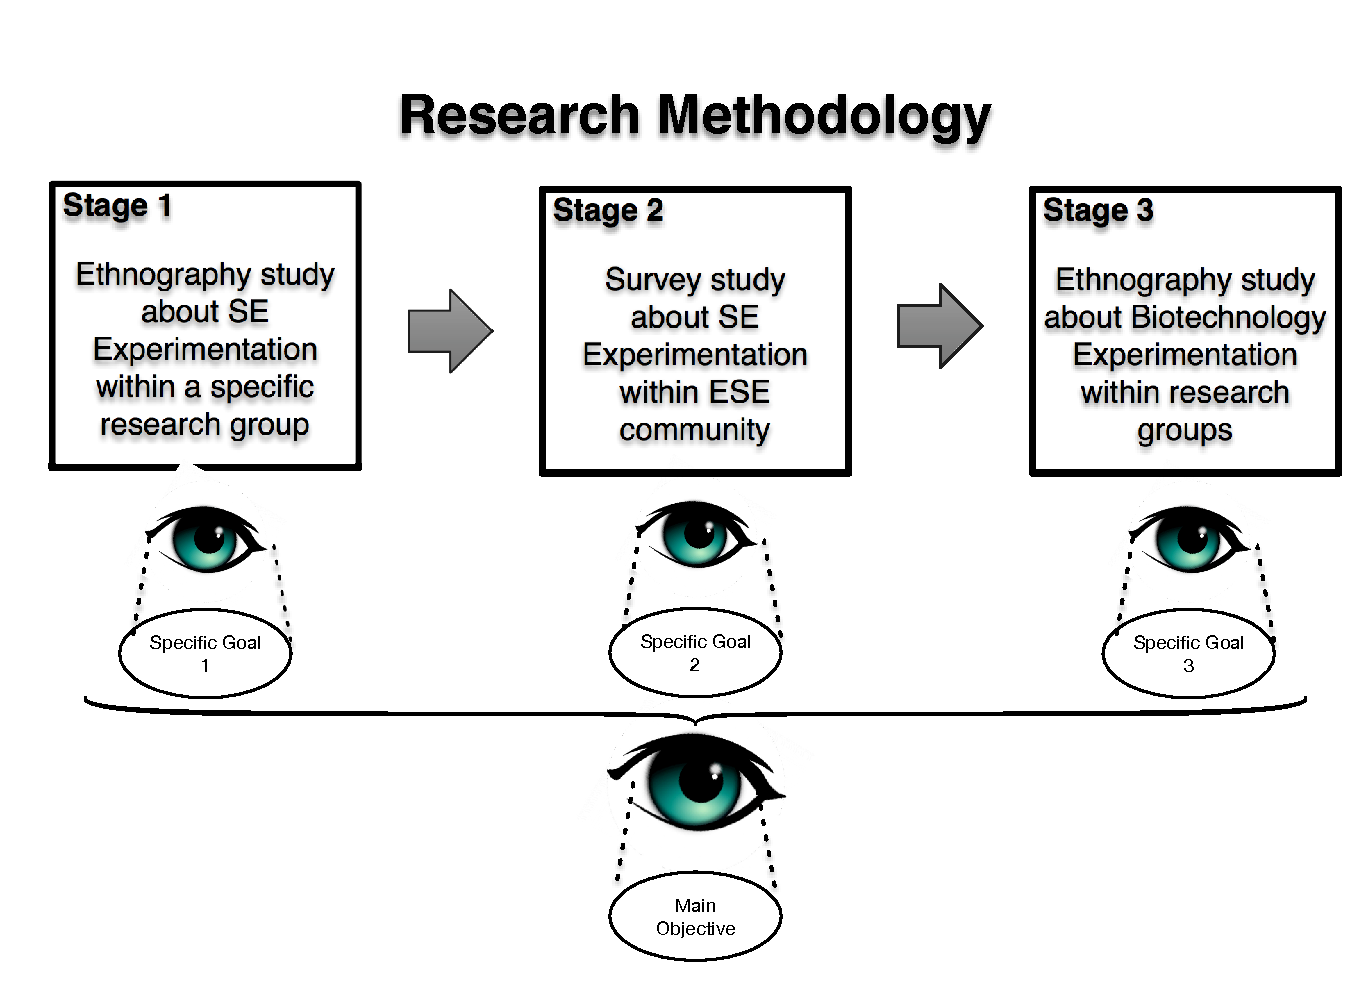
\includegraphics[width=10cm]{Images/Methodology}
	\caption{Research Methodology}
	\label{fig-research-methodology}
\end{figure*}

Los estudios etnogr�ficos pretenden dar respuesta a dos preguntas de investigaci�n concretas:

\begin{framed}%
\textbf{RQ1: How researchers conduct the SE experiments in practice into a specific research group?}
\end{framed}

\begin{framed}%
\textbf{RQ2: Is there deviation of the SE experimentation practice from traditional disciplines?}
\end{framed}

Para responder rigurosamente a estas preguntas, ser�a preciso realizar la investigaci�n en varias muestras del universo de grupos de investigaci�n de ambas disciplinas. Dado el alto costo que esto representa, la �nica alternativa factible ser�a la realizaci�n de un survey. Sin embargo, un survey podr�a sesgar la respuesta a las preguntas de investigaci�n, i.e., los experimentadores podr�an reportar lo que creen que hacen, en lugar de lo que realmente hacen. Este efecto ya ha sido observado anteriormente [REF].
 
Visto desde esta perspectiva, se precis� aplicar una aproximaci�n emp�rica de observaci�n para garantizar la fiabilidad de los resultados obtenidos, su validez y significancia cient�fica \cite{sjoberg-2007-future-empical-methods}. Por lo tanto, los m�todos factibles a ser utilizados eran: etnograf�a, action research o case study. Como esta investigaci�n precisaba estudiar c�mo se desarrolla la experimentaci�n en su entorno natural (grupos de investigaci�n), realizamos los ethnographical studies \cite{Sharp-2016-Ethnographic-Studies-ESE}.

Esta metodolog�a obliga a que la investigaci�n sea llevada a cabo en un peque�o n�mero de grupos de investigaci�n, lo que implica ciertos riesgos, dado que la validez de los resultados se ve amenazada. Para disminuir estos riesgos llevamos a cabo un riguroso proceso investigativo en contextos de experimentaci�n (i.e., grupos de investigaci�n) representativos de la poblaci�n bajo estudio (i.e., experimentadores en ESE y otra disciplina experimental asentada). Para aumentar la validez de nuestro estudio, triangulamos los resultados de la investigaci�n etnogr�fica con el survey antes citado, lo que nos permiti� responder a la siguiente pregunta de investigaci�n:

%\begin{framed}%
%\textbf{RQ3: To determine the generalizability of the experimentation process performed into a specific SE research group}
%\end{framed}

\begin{framed}%
\textbf{RQ3: �Cu�n generalizables son nuestros hallazgos a la comunidad de experimentadores en SE?}
\end{framed}

\subsection{Ethnographical Studies}
Los estudios etnogr�ficos se estructuraron en base a las gu�as de Per Runenson \cite{Runenson-2012-case-study-in-SE} para estudios de caso. Estas gu�as dan un soporte bastante espec�fico para las investigaciones que pretenden entender fen�menos que suceden en el mundo real; no obstante, es preciso tener presente que hacer una investigaci�n exhaustiva de este tipo en SE, no es una tarea f�cil.

El dise�o de los estudios etnogr�ficos consisten de: (1) Context selection, (2) Data collection procedures, y (3) Data analysis procedure.

\subsubsection{Context selection}
El criterio de selecci�n del contexto aplicado en los estudios etnogr�ficos parte de la premisa que un grupo de investigaci�n representativo constituye una fuente fiable de informaci�n, lo que facilita la tarea de aprendizaje respecto a la experimentaci�n. Por lo tanto, planteamos las siguientes condiciones como criterios de selecci�n del contexto:

\begin{itemize}
\item{Ser un grupo de investigaci�n cuyos experimentadores tengan una consolidada experiencia en el �rea}

\item{Ser un grupo de investigaci�n cuyos experimentadores sean reconocidos en la comunidad cient�fica a trav�s de publicaciones de alto impacto, tales como libros, art�culos, manuales t�cnicos, entre otras.)}
\end{itemize}

Dadas estas condiciones, los grupos seleccionados son, por una parte, el Grupo de Investigaci�n en Ingenier�a de Software Emp�rica (GrISE) perteneciente a la Escuela T�cnica Superior de Ingenieros Inform�ticos (ETSII) de la Universidad Polit�cnica de Madrid (PM) de Espa�a y por otra parte, tres grupos de investigaci�n de la Carrera de Biotecnolog�a de la Universidad de las Fuerzas Armadas ESPE de Ecuador. Una descripci�n detallada de los grupos de investigaci�n seleccionados se realiza en las Secciones \ref{sec-ESE-etnography} y \ref{sec-bio-etnography}, respectivamente.

\subsubsection{Data collection procedures}\label{subsec-data-collection}
El proceso de recolecci�n de informaci�n aplicado fue c�clico, iterativo e incremental, cuyas acciones fueron realizadas sobre distintas fuentes de informaci�n, con el prop�sito de indagar sobre la experimentaci�n llevada a cabo en los grupos de investigaci�n seleccionados.

Las fuentes generadoras de informaci�n corresponden espec�ficamente a aquellas accesibles y representativas dentro de los grupos de investigaci�n bajo estudio. Para la presente investigaci�n se consider� (en los casos que fue posible) a la: Literatura com�n del grupo (general y espec�fica), material experimental del grupo (general y espec�fico) y conocimiento de los experimentadores del grupo (internos y externos).

El orden en el que el investigador toma contacto con las fuentes de informaci�n es aleatorio. La frecuencia de contacto con las fuentes depende de la necesidad del investigador por cumplimentar el conocimiento; pero sobre todo, depende de la disponibilidad de cada fuente. Es decir, mientras m�s disponible es la fuente, el investigador se mantiene m�s tiempo en contacto con la misma. A continuaci�n se detalla la interacci�n del investigador con cada fuente.

\begin{itemize}
  \item En lo que respecta a la literatura com�n del grupo, el investigador tiene acceso a la misma de forma inmediata y continua en el tiempo, a trav�s de bibliotecas, bases digitales disponibles, versiones impresas disponibles, entre otras. La literatura representa una fuente de informaci�n muy importante, dado que proporciona la informaci�n referente al proceso de experimentaci�n, desde la perspectiva te�rica.
 
  \item El contacto con el material experimental m�s representativo y fiable propio del grupo de investigaci�n es inmediato y continuo en el tiempo, con la gu�a de los experimentadores. Sin embargo, para facilitar el proceso de revisi�n y aprendizaje de la informaci�n contenida en esta fuente, se precisa un contacto previo con la literatura com�n del grupo. Eventualmente es preciso el estudio de material espec�fico para profundizar en una tem�tica particular. El material experimental representa la evidencia de la experimentaci�n llevada a cabo en la pr�ctica por el grupo de investigaci�n.

  \item La obtenci�n del conocimiento de los experimentadores es planificada en funci�n de su disponibilidad de tiempo. Este proceso se realiza desde un inicio, ya que se representa una alta complejidad, considerando la aplicaci�n de distintas t�cnicas e instrumentos. Para el caso de los experimentadores externos, no es posible una planificaci�n espec�fica, dada la dificultad de un contacto directo; por lo tanto, en este punto mucho se depende de la casualidad. El conocimiento obtenido de los experimentadores, representa el proceso de experimentaci�n realizado en la practica dentro de los grupos de investigaci�n. 
\end{itemize}

El conocimiento obtenido de las fuentes indicadas se complement� entre si y sirvi� para determinar en qu� medida lo que se encuentra expresado en la teor�a, corresponde a lo que efectivamente llevan a cabo los experimentadores en la pr�ctica dentro de los grupos de investigaci�n.

Para el proceso de extracci�n de la informaci�n se utiliz� una taxonom�a de t�cnicas de recolecci�n de informaci�n, categorizada de acuerdo al nivel de contacto con la fuente primaria de informaci�n. La taxonom�a propone tres niveles de recolecci�n de informaci�n: Participaci�n directa con la fuente (nivel 1), participaci�n indirecta con la fuente (nivel 2) y estudio del material de trabajo (sin la participaci�n de la fuente) (nivel 3) \cite{Lethbridge-2005-studyingsoftwaredatacollection}.

El procedimiento para la recolecci�n de informaci�n de las fuentes indicadas, consiste en aplicar t�cnicas adecuadas dependiendo del tipo de fuente y de su disponibilidad. Por ejemplo, para extraer informaci�n de los experimentadores de un entorno de experimentaci�n se utilizaron t�cnicas tales como: entrevistas, grupos de discusi�n, entre otros (primer nivel). La adecuada aplicaci�n de las t�cnicas de recolecci�n de informaci�n se asocia a la utilizaci�n de diferentes instrumentos, algunos de los cuales se constituir�n como piezas fundamentales para recrear la informaci�n obtenida. Por ejemplo utilizamos: videoc�maras, dispositivos de grabaci�n de audio, entre otros. M�s espec�ficamente, las t�cnicas de recolecci�n de informaci�n aplicadas a las fuentes de informaci�n, se indican en la Tabla \ref{tbl-tecnica-fuente}.

\begin{table}
	\centering
	\caption{T�cnicas de recolecci�n por fuente de informaci�n}
	\label{tbl-tecnica-fuente}
	\begin{tabular}{|p{3.7cm}|p{3.7cm}|}
	\hline
	\textbf{Fuente} & \textbf{T�cnicas}\\
	\hline
	\multirow{7}{50 pt}{Conocimiento del grupo de investigaci�n} & Entrevistas\\
	\cline{2-2}
	& Grupos de discusi�n\\
	\cline{2-2}
	& Observaci�n participativa\\
	\cline{2-2}
	& Modelado de actividades\\
	\cline{2-2}
	& Sistemas instrumentales\\
	\cline{2-2}
	& Aprendizaje basado la experiencia\\
	\hline
	\multirow{1}{85 pt}{Literatura referente} & An�lisis de documentaci�n\\
	\hline
	\multirow{1}{95 pt}{Material experimental} & An�lisis de documentaci�n\\
	\hline
	\multirow{3}{95 pt}{Conocimiento de experimentadores} & Entrevistas\\
	\cline{2-2}
	& Grupos de discusi�n\\
	\cline{2-2}
	& Sistemas instrumentales\\
	\hline
	\end{tabular}
\end{table}
 
Los inconvenientes presentados por el uso de las diferentes t�cnicas e instrumentos fueron minimizados gracias a su combinaci�n en cada iteraci�n. Por ejemplo, los vac�os del audio fueron complementados por el video, las fotograf�as y los esbozos de los experimentadores y viceversa.

\subsubsection{Data analysis procedure}
El procedimiento de an�lisis de datos tiene un enfoque cualitativo y est� asociado con la aplicaci�n de las t�cnicas de obtenci�n de informaci�n, por lo que fue iterativo incremental. El n�mero de iteraciones de an�lisis corresponde al n�mero de iteraciones de recolecci�n de datos realizado con cada fuente. El procedimiento de an�lisis (ver Figura \ref{fig-proc-analisis}) se compone de dos actividades principales: (1) Verificaci�n de los datos y (2) Comparaci�n de los datos.

\begin{figure}[htbp!]
	\centering
	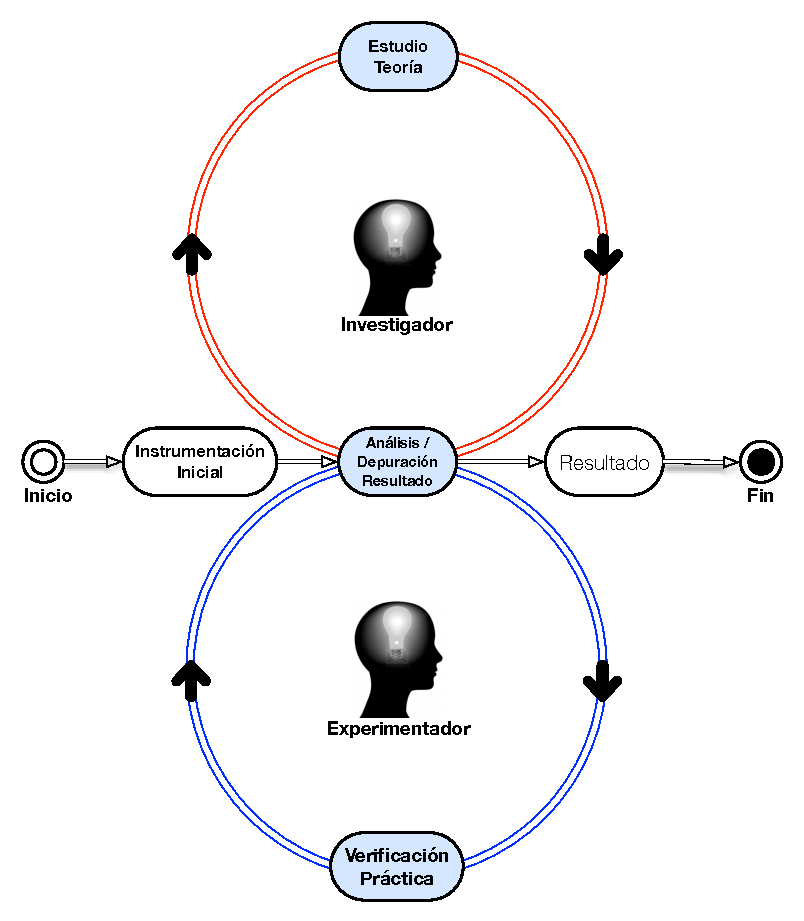
\includegraphics[width=2.5in]{Images/proceso-analisis}
	\caption{Proceso de An�lisis}
	\label{fig-proc-analisis}
\end{figure}

La actividad de verificaci�n de datos tiene como prop�sito verificar la validez de la informaci�n recolectada como insumo para el an�lisis, lo cual ser� realizado principalmente por los mismos experimentadores del grupo bajo estudio. Durante las revisiones de las fuentes te�ricas, los investigadores fueron adquiriendo paulatinamente conocimientos b�sicos de la experimentaci�n, lo cual les sirvi� para entender m�s f�cilmente los resultados obtenidos de la interacci�n con el conocimiento de los experimentadores. Los resultados obtenidos fueron expresados de forma expl�cita en medios f�sicos o digitales y validados por los experimentadores en cada iteraci�n hasta obtener el resultado final.
 
Comparaci�n de los datos: La comparaci�n de los datos obtenidos fue realizada tanto por los investigadores como por los experimentadores en una actividad de revisi�n cruzada, cada vez que se realiz� la verificaci�n de los datos en los resultados intermedios obtenidos. Por un lado los investigadores hacieron la comparaci�n del resultado con su conocimiento adquirido de la revisi�n de otras fuentes de informaci�n; mientras que los experimentadores compararon el resultado con las actividades que efectivamente realiza en la pr�ctica.

\subsection{Survey of the experimentation process in SE}
Para validar los hallazgos del estudio sobre el proceso de experimentaci�n en SE dentro de un grupo de investigaci�n, realizamos un survey en la comunidad de ESE. Siguiendo los 

\subsubsection{Introduction}
This research is intended to study the underlying problems surrounding the ESE and inquire about their possible origins. To do this, we carried out an empirical study based on a structured survey, in order to obtain insight of the most representative researchers into the Empirical Software Engineering Community. From this point of view, we have considered survey the researchers whose articles have been accepted in the most representative symposiums, workshops or conferences, such as: the ``Symposium on Empirical Software Engineering and Measurement" (ESEM), the Experimental Software Engineering Latin America Workshop (ESELAW), among others.

\subsubsection{Survey's Goal}
This research aims to study the underlying problems surrounding the Experimentation in Software Engineering and find out their possible origins. This study will be carried out through a structured survey in the context of the ESEM and ESELAW symposiums.

With the purpose of contextualize the survey's goal, the following research questions were proposed.

\begin{framed}%
\textbf{RQ1: What are the circumstances in which SE researchers obtained their base training on experimentation and what is their current experience?}
\end{framed}

\begin{framed}%
\textbf{RQ2: How is the experimental process in Software Engineering?}
\end{framed}

\begin{framed}%
\textbf{RQ3: What problems are faced by researchers during experimental software engineering process?}
\end{framed}

\begin{framed}%
\textbf{RQ4: What instances of experimental process need improvement from the point of view of Software Engineering researchers?}
\end{framed}

\subsubsection{Target Population}
Software Engineering researchers whose papers were accepted in ESEM 2016 symposium, and researchers who usually published in the CIbSE conference's track named ESELAW.

\subsubsection{Sampling Design}
The website (based on a survey) used to operationalize the study will be published through flyers and email to our target population. Advertising aims to capture the attention of researchers to implement the survey.

\subsubsection{Survey's Questions}



\section{Experimentation In Software Engineering}\label{sec-ESE-etnography}
El estudio fue realizado en el Grupo de Investigaci�n en Ingenier�a de Software Experimental (GrISE) de la Universidad Polit�cnica de Madrid (UPM). GrISE es un grupo que puede considerarse representativo de la comunidad de ESE. El origen del grupo data de finales de los 90s, cuando fue fundado por N. Juristo, una investigadora reconocida en IS por su temprano libro acerca de SE experimental \cite{Juristo2001} (con A. Moreno), adem�s de sus contribuciones posteriores. El grupo cuenta con otros investigadores de dilatada trayectoria, tales como Oscar Dieste y Sira Vegas. A lo largo de su historia, GrISE ha realizado varias familias de experimentos \cite{Basili1999-KnowledgeFamiliesExp}, en distintas tem�ticas: testing, requisitos y, m�s recientemente, test-driven development.

\subsection{First Approximation}\label{subsec-results-case1}
Los primeros contactos con el grupo de investigaci�n tuvieron lugar en 2012. Nuestra pretensi�n inicial era adquirir el conocimiento del grupo y volcarlo en modelos conceptuales, de una forma similar a la pr�ctica de la ingenier�a del conocimiento.

En un primer momento la tarea pareci� factible. Los miembros del GrISE hac�an continuas referencias a fuentes de consulta que ellos consideraban est�ndar, como por ejemplo el texto: \textit{Experimentation in Software Engineering} by Wohlin et al. \cite{Wohlin2012-Experimentation}; e igualmente a su material experimental, como por ejemplo a los: planteamientos de experimentos. Las primeras acciones de nuestra parte a llevar a cabo estaban claras: el estudio de la literatura preferida por el grupo y el estudio de su material experimental.

Sin embargo, pronto se evidenci� una barrera de entrada en el acceso al grupo: aunque el discurso del grupo era claramente general (e.g., nos hablaban de \textit{objetos experimentales} tal y como eran considerados en la literatura), su referente era eminentemente local (referido espec�ficamente a, material usado previamente por los miembros del grupo e.g., los programas usados en la familia de experimentos de testing). Esto dificultaba enormemente nuestra comprensi�n del modo en que el grupo llevaba a cabo su investigaci�n, confirm�ndose as� la necesidad de estudiar, adem�s de los textos est�ndar, tambi�n la literatura espec�fica del grupo.

\subsubsection{Review Of Preferred Literature}\label{subsubsec-study-literature}
Los miembros del GrISE se�alaron como fuentes b�sicas acerca de experimentaci�n en SE a los libros: \textit{Experimentation in Software Engineering} by Wohlin et al. \cite{Wohlin2000} and \textit{Basics of Software Engineering Experimentation} by Juristo et al. \cite{Juristo2001}. Ambos libros son probablemente los mejor conocidos \cite[p.~3]{Wohlin-2007-ESE-Teaching-Methods}, en parte tambi�n porque los textos de referencia son muy escasos. Tambi�n mencionaron de forma preferente los estudios: \textit{Building Knowledge Through Families of Experiments} \cite{Basili1999-KnowledgeFamiliesExp}, el cual parece una preferencia espec�fica del GrISE, dado su inter�s particular por realizar replicaciones experimentales; \textit{Experimentation in Software Engineering} \cite{Basili-1986-ESE}, el cual representa una de las primeras gu�as acerca de como llevar a cabo experimentos en SE; and \textit{Preliminary Guidelines for Empirical Research in Software Engineering} \cite{Kitchenham2002-GuideLinesESE}, las cuales son unas de las recomendaciones seminales acerca de como experimentar en SE.

Las fuentes anteriores fueron revisadas en profundidad por dos investigadores (E. Fonseca y E. Espinosa), quienes al momento en que se realiz� el estudio, contaban �nicamente con una formaci�n en ingenier�a tradicional y una especializaci�n en SE. Esta situaci�n les permiti� abstraer los fundamentos de la SE experimental, que hasta ese entonces era un contexto totalmente desconocido para ellos; tal cual etn�grafos de principio de siglos visitando las tribus de �frica para entender sus costumbres y crear conocimiento de lo desconocido \cite{Aman-1978-africa-ethnography}.

En definitiva, los libros y art�culos estudiados propiciaron la adquisici�n del conocimiento espec�fico referido a conceptos tales como: Experimento, Replicaci�n, S�ntesis, Hip�tesis, Variables, Dise�o Experimental, etc. Al mismo tiempo, comenzamos a organizar dichos conceptos en un modelo conceptual preliminar, tal y como muestra la figura \ref{fig-conceptos-preliminar}.

\begin{figure}[htbp!]
	\centering
	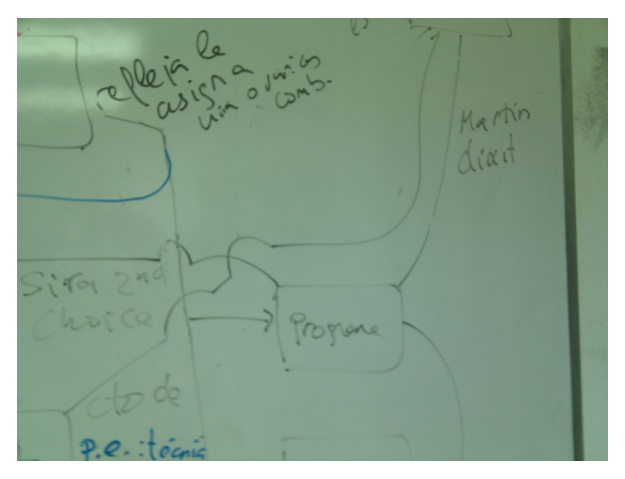
\includegraphics[width=3in]{images/Concept-Draft}
	\caption{Extracto del Modelo Conceptual Preliminar de la Experimentaci�n en GrISE}
	\label{fig-conceptos-preliminar}
\end{figure}

El primer aspecto que nos llam� la atenci�n fue la \textit{diversidad terminol�gica con que las distintas fuentes se refer�an a actividades similares del proceso experimental}. Para un observador sin conocimientos del �rea, la literatura parecer�a describir distintos tipos de experimentos, cada uno caracterizado por un proceso diferente. Una vez adquiridos los conocimientos b�sicos acerca de la materia, es inmediato percibir las similitudes, pero a�n as� no est� claro si los distintos autores est�n describiendo exactamente a las mismas actividades. Esto no ocurre solo a nivel de libros de texto, lo cual podr�a ser esperable, \textit{sino que tambi�n se extiende a otros materiales, tales como recomendaciones de reporte y art�culos}.

Podemos citar como ejemplos de la diversidad terminol�gica encontrada, a la denominaci�n heterog�nea utilizada por algunos autores para las fases del proceso de experimentaci�n en SE, tal como se indica a continuaici�n.

\begin{itemize}
	\item Juristo \& Moreno \cite{Juristo2001} proponen como fases del proceso a \textquotedblleft Objective Definition, Design, Execution and Analysis\textquotedblright.
	\item Wohlin et al. \cite{Wohlin2000} \textquotedblleft Experiment idea, Experiment scoping, Experiment planning, Experiment operation, Analysis \& interpretation, Presentation \& package and Experiment report\textquotedblright.
	\item Basili et al. \cite{Basili-1986-ESE} propose \textquotedblleft definition, planning, operation, and interpretation\textquotedblright.
\end{itemize}

Aunque los autores definen estas fases m�s en detalle en funci�n de las actividades que incluye cada una, la coincidencia en t�rminos y descripci�n difiere mucho de uno a otro autor.

Despu�s de buscar libros de texto complementarios a los indicados anteriormente, con la intenci�n de verificar si la diversidad terminol�gica era un problema general, o estaba circunscrito a las fuentes recomendadas, solo hemos localizado la nueva edici�n de Wohlin et al. \cite{Wohlin2012-Experimentation} sobre experimentaci�n y los libros especializados de Runeson et al. \cite{case-study-in-SE-Runenson-2012} y Kitchenham et al. \cite{Kitchenham-2015-Literature-Review-Book}. Preguntados a este respecto a los miembros del GrISE, nos se�alaron adicionalmente otras fuentes, tales como Box et al. \cite{Box2008} o Montgomery \cite{montgomery-2010-applied-statistics}, las cuales pertenecen al �rea de ingenier�a, pero no a la de experimentaci�n en SE. Por lo tanto, la \textit{carencia de textos sobre experimentaci�n en SE} es es otro aspecto noticeable. 

Esta situaci�n acrecent� nuestra convicci�n respecto a que la \textit{diversidad terminol�gica} pudiera ser todav�a mayor de la observada, incluyendo tambi�n una \textit{diversidad de aproximaciones y enfoques sobre la realizaci�n de experimentos}.

\subsubsection{Review of experimental material}\label{subsubsec-study-material}
El material experimental del grupo GrISE se compone fundamentalmente de: planteamientos de experimentos, dise�os experimentales, art�culos (e.g.: \cite{Juristo2012-EffectivenessWithinOutsideScopeExperiment,Juristo2006-SoftwareTestingTechniques,Juristo-2003-ESERNET}), instrumentos experimentales (e.g.: formularios de tareas experimentales, formularios de recogida de datos, gu�as), objetos experimentales (e.g.: programas con faltas sembradas, especificaciones de requisitos con anomal�as), raw data (e.g.: hojas de excel con datos de mediciones de tareas experimentales realizadas, bases de datos) y material de entrenamiento (e.g.: manuales t�cnicos \cite{Juristo2006-SoftwareTestingTechniques}, presentaciones).

El primer problema que nos encontramos fue el mismo acceso al material experimental, dado que \textit{no existe una pol�tica o herramienta para la gesti�n del material}. Un ejemplo paradigm�tico son los raw data. Encontramos raw data en distintos tipos de ficheros, correspondientes a distintas versiones, cuya ubicaci�n y formato son conocidos solo por la persona que los gestiona. Lo mismo puede afirmarse, aunque en menor medida, de los restantes tipos de materiales (e.g.: instrumentos u objetos experimentales); con la excepci�n de las publicaciones, las cu�les son f�cilmente accesibles en las librer�as digitales.

Fue preciso solicitar ayuda a los miembros del GrISE para acceder al material experimental, entender su estructura y la forma de gesti�n particular que utilizan. La revisi�n se realiz� de forma progresiva en funci�n de su antig�edad (i.e., primero revisamos lo m�s antiguo y luego lo m�s actual). Todas las fases de revisi�n siempre fueron guiadas por el albacea de la informaci�n, cuyo relato sumado a la informaci�n obtenida del material revisado, nos permiti� descubrir que  \textit{las actividades que generaron el material experimental han ido evolucionando y mejorando con el tiempo}. Por ejemplo, nos indicaron que los reportes experimentales, a pesar de haber sido aceptados en congresos y revistas de alto impacto, han ido perfeccion�ndose con el tiempo, sobre todo porque la exigencia de los revisores se ha incrementado.

Otro aspecto que nos llam� la atenci�n en la revisi�n del material experimental, fue \textit{la extensi�n (entre 100 a 120 p�ginas) y complejidad del planteamiento de los experimentos}. Estos documentos se caracterizan por tener una \textit{descripci�n general de las actividades a ser realizadas en el experimento}, lo cual dificulta entender las particularidades que conlleva un experimento en la pr�ctica; por otra parte, \textit{no dan una gu�a sobre el orden de ejecuci�n de las actividades experimentales}. Encontramos planteamientos de experimentos que inclu�an un dise�o experimental, mientras que otros no. Aquellos planteamientos con dise�o experimental, no especifican el tipo de dise�o que utilizan, solo indican su estructura y conformaci�n; adicionalmente, estos dise�os hac�an referencia a t�rminos totalmente diferentes a los identificados hasta el momento, y por ende dif�ciles de comprender, tales como: \textit{efecto del cansancio}, \textit{efecto del aprendizaje}, etc. Aunque en este punto cre�mos tener cierto nivel de conocimiento sobre la experimentaci�n en SE, las \textit{inconsistencias encontradas entre las fuentes revisadas}, acrecentaron nuestra \textit{incertidumbre sobre la fiabilidad de dichas fuentes}; por lo tanto, se torn� imperiosa la necesidad de revisar fuentes adicionales para contrastar lo encontrado hasta el momento e intentar incrementar y afianzar el conocimiento alcanzado.

\subsection{Understanding The Experimental Process in SE}\label{subsec-second-aprox}
El estudio del material experimental propio del grupo constituy� sin duda una fuente de informaci�n fundamental para averiguar c�mo GrISE se enfrenta a la experimentaci�n, m�xime cuando refleja probablemente una gran cantidad de conocimiento t�cito del grupo, gestado sobre la base de m�s de una d�cada de experimentaci�n. Sin embargo, el conocimiento contenido en el material experimental no fue posible abstraerlo, dado que \textit{no presentaba una gu�a clara de c�mo hacer un experimento}; en este punto, la alternativa te�rica perdi� su atractivo y fue tiempo de pensar en la pr�ctica. Por lo tanto, consideramos que la ejercitaci�n con el material experimental, de la mano de la gu�a de los miembros del GrISE, constituir�a el camino a la familiarizaci�n de su formato, uso, e incluso verificaci�n de resultados; pero que especialmente, podr�a permitirnos la habituaci�n con actividades propias de la experimentaci�n, tales como: c�lculo de medidas a partir de la raw-data contenida en los materiales, formateo de la raw-data para an�lisis estad�stico, reproducci�n de resultados estad�sticos a partir de las mediciones, recreaci�n de gr�ficos y tablas estad�sticas a partir de las mediciones, etc. M�s espec�ficamente, consideramos la posibilidad de seleccionar el material de un experimento particular, para intentar recrearlo y aprender de la pr�ctica en un entorno real.

\subsubsection{Review of Specific Experimental Material}\label{subsubsec-review-specific-material}
Con la ayuda de los miembros del GrISE, ubicamos el material de un experimento espec�fico para su estudio y posterior replicaci�n en un contexto real. El principal prop�sito de este ejercicio fue el de aprender de la experimentaci�n en la pr�ctica. Puntualmente, realizamos la replicaci�n \cite{Fonseca-2013-Replication-Efectiveness-In-Out} del experimento de t�cnicas de pruebas de software de Juristo et al. \cite{Juristo2012-EffectivenessWithinOutsideScopeExperiment} en la Universidad de la Fuerzas Armadas ESPE, Sede Latacunga, de Ecuador.

\textit{Realizar en la pr�ctica una replicaci�n experimental sin duda permiti� entender de forma m�s did�ctica su proceso completo y las actividades inherentes}, e igualmente permiti� \textit{validar el conocimiento obtenido en la revisi�n de la literatura referente y del material experimental del GrISE}. El hallazgo m�s importante de esta actividad fue \textit{comprobar la dificultad que representa llevar a cabo un experimento en la pr�ctica, m�s a�n al tratar de recrear fielmente un experimento ya realizado en un entorno diferente}. Es preciso mencionar que la replicaci�n en sus fases iniciales cont� con la participaci�n directa de los investigadores que realizaron el experimento original, en este caso los mismos miembros del GrISE; cuyo aporte principal fue guiar el dise�o experimental, el uso del material experimental y dar los lineamientos espec�ficos para realizar la ejecuci�n y an�lisis del experimento.
 
 No obstante, los resultados de la replicaci�n tuvieron diferencias marcadas con respecto al experimento original, posiblemente por factores propios del contexto donde se llev� a cabo la replicaci�n, o por falta de experiencia de quienes la ejecutaron. Esto indica que ap parecer el conocimiento m�s granular sobre la ejecuci�n del experimento no fue abstra�do del todo por quienes realizaron la replicaci�n en el contexto real.

Evaluando las actividades realizadas hasta el momento en la investigaci�n, encontramos que posiblemente el contenido de los textos de experimentaci�n revisados representen de forma expl�cita una parte del conocimiento de sus autores; sin embargo, comparando dicho contenido con los elementos del material experimental del GrISE, y con las actividades que no estaban indicadas en el material espec�fico revisado, y que nos fueron aclaradas para poder realizar la replicaci�n, vimos que las diferencias son muy marcadas, lo que muestra \textit{la generalidad de los textos, la falta de detalle del material experimental y por ende la presencia de un conocimiento t�cito particular de cada investigador}; esto justifica la gu�a permanente que tuvimos de los miembros del GrISE. Sin duda alguna las aproximaciones realizadas nos permitieron adquirir un conocimiento muy general de la experimentaci�n en IS; no obstante, el conocimiento m�s granular del proceso experimental segu�a perteneci�ndole a los investigadores del GrISE. Por lo tanto, fue preciso volver al principio y enfocarnos en dicho conocimiento.

\subsection{The Real Source Of Knowledge Regarding The Experimental Process in Software Engineering}\label{subsec-conocimiento-grupo}
Nuestra intenci�n en este punto fue debelar la incertidumbre sobre el origen de la diversidad terminol�gica y operativa entorno al proceso experimental en SE; para lo cual, pretendimos hacer expl�cito en un alto porcentaje el conocimiento granular de la experimentaci�n en SE que poseen los miembros del GrISE, lo cual, seg�n nos indicaron, no hab�a sido realizado anteriormente. Por lo tanto, planificamos estudiar a cada miembro como fuente directa de informaci�n, para lo que nos fueron concedidas de forma paralela entrevistas personales y reuniones grupales de discusi�n.

\subsubsection{Interviews With GrISE Members}\label{subsubsec-interviews}
Las entrevistas a los miembros del GrISE se sustentaron en un cuestionario simple de preguntas abiertas para conocer a detalle las actividades que lleva a cabo cada miembro dentro del proceso experimental del GrISE. El cuestionario se enfoc� en motivar al entrevistado en un relato libre y abierto sobre las actividades puntuales que realiza. En las primeras sesiones se afin� la t�cnica de abstracci�n de conocimiento para obtener el mayor detalle posible. Por ejemplo, se pas� de utilizar papel y l�piz para tomar nota de las respuestas de los entrevistados, a grabaciones de audio y video, con lo cual se agiliz� el proceso y sobre todo se pudo captar los detalles m�s granulares referidos a lo expresado, a los gestos, e incluso de los rasgos con los que algunos entrevistados esbozaban su relato con pluma y papel (por ejemplo ver Figura \ref{fig-proceso-exp-boseto}).

\begin{figure}[htbp!]
	\centering
	\includegraphics[width=3.2in]{images/Boseto-Proccess}
	\caption{Extracto de las actividades experimentales realizadas por los experimentadores del GrISE en boceto}
	\label{fig-proceso-exp-boseto}
\end{figure}

El conocimiento abstra�do en cada sesi�n de entrevistas fue validado con el investigador entrevistado al inicio de la sesi�n posterior; lo cual fue presentado al entrevistado en formato impreso compuesto en la mayor�a de los casos por texto, a diferencia de de la entrevistados a la fundadora del grupo, quien adicion� en su relato un boceto sobre las actividades del proceso experimental, el cual fue recreado con herramientas inform�ticas.

Los resultados de las entrevista, especialmente aquellos que incluyeron una descripci�n gr�fica del proceso experimental, mostraron que \textit{los experimentadores de mayor experiencia tienen un conocimiento m�s amplio y detallado sobre las actividades que llevan a cabo en la experimentaci�n en SE}.

El proceso de entrevistas fue iterativo y permiti� generar productos intermedios del proceso experimental, tanto en relato escrito como gr�fico (por ejemplo ver Figura \ref{fig-proceso-draft}) y termin� tanto en cuanto el entrevistado indicaba que su relato sobre las actividades que realiza en el proceso experimental hab�a concluido y estaba de acuerdo con el producto final obtenido (por ejemplo ver Figura \ref{fig-proceso-exp}). Una situaci�n particular que nos llam� la atenci�n fue que \textit{el detalle de actividades obtenido en el flujograma de la Figura \ref{fig-proceso-exp} parece indicar que los pocos textos sobre experimentaci�n en SE existentes, est�n lejos de mostrar el trabajo real que implica la experimentaci�n en la pr�ctica de principio a fin.}

\begin{figure}[htbp!]
	\centering
	\includegraphics[width=3.2in]{images/Proccess-Draft}
	\caption{Extracto de las actividades experimentales realizadas por los experimentadores del GrISE (versi�n intermedia)}
	\label{fig-proceso-draft}
\end{figure}

\begin{figure}[htbp!]
	\centering
	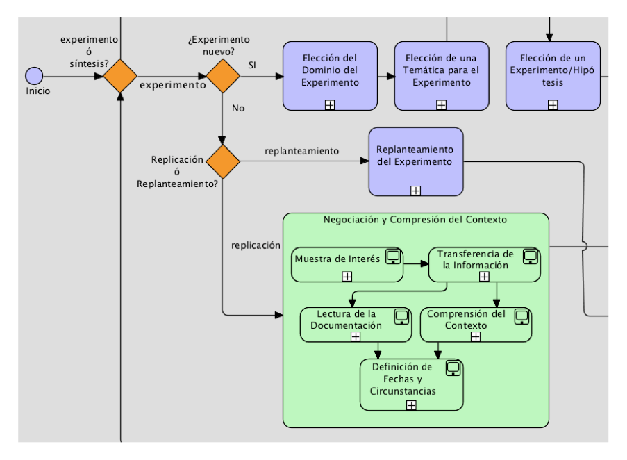
\includegraphics[width=3.2in]{images/Proccess}
	\caption{Extracto de las actividades experimentales de SE realizadas por los experimentadores del GrISE (versi�n final)}
	\label{fig-proceso-exp}
\end{figure}


Sin embargo, los resultados tambi�n mostraron que \textit{las actividades realizadas por los experimentadores entrevistados difieren de un experimentador a otro, de hecho ning�n experimentador entrevistado lleva a cabo todas las actividades identificadas de la experimentaci�n en SE.} Ante esto fueron consultados los miembros del GrISE e indicaron que \textit{no existe una definici�n explicita para el grupo actividades que realiza cada experimentador}; de hecho, ese momento acordaron identificar 3 grupos de actividades espec�ficas o roles que realizaban los miembros del GrISE y los denominaron: Research Manager, Experiment Manager and Senior Experimenter, los cuales se encargan de planificar la ejecuci�n del experimento, ser el albacea de la informaci�n y gestionar la log�stica de la experimentaci�n, respectivamente.

Entre los grupos de actividades identificados, \textit{existen actividades experimentales que son ejecutadas por duplicado en una misma instancia experimental. Como por ejemplo: Gesti�n de la replicaci�n experimental, planteamiento del experimento, entre otras}.

\subsubsection{Focus Groups With GrISE Members}\label{subsubsec-focus-groups}
La t�cnica de Focus Groups se apoy� en las mismas t�cnicas e instrumentaci�n de la entrevista, con el prop�sito de que los miembros del equipo de trabajo puedan esbozar y participar en el modelado conceptual de la experimentaci�n en SE, el investigador participe activamente en el debate sobre las propuestas de los experimentadores y el investigador cubra inquietudes menores con el experimentador sin tener necesariamente contacto personal.

\textbf{Focus Groups sobre los conceptos manejados en la experimentaci�n en SE}\\
El proceso de Focus Groups sobre la terminolog�a manejada en la experimentaci�n en SE fue c�clico. Se parti� de un boceto creado en consenso por los experimentadores en la pizarra (ver Figura \ref{fig-conceptos-draft}), luego de lo cual se realizaron varias sesiones de focus groups. En cada instancia de Focus Groups se gener� un producto intermedi�, el cual fue validado por el grupo en la siguiente sesi�n, hasta obtener el producto final (ver Figura \ref{fig-conceptos-exp-boseto}).

\begin{figure}[htbp!]
	\centering
	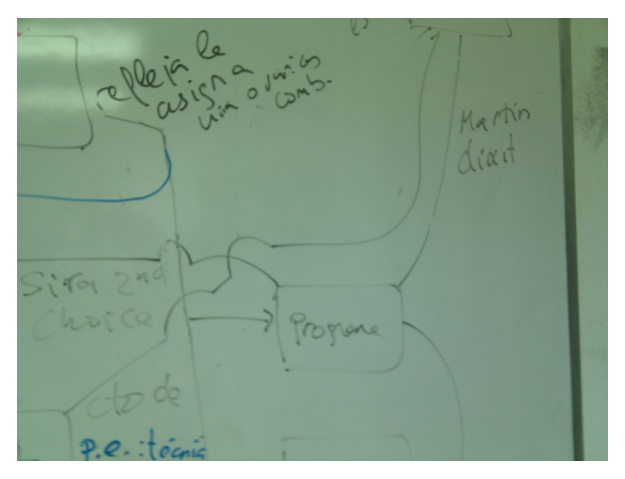
\includegraphics[width=3in]{images/Concept-Draft}
	\caption{Extracto del Modelo Conceptual de la Experimentaci�n en GrISE en Boceto}
	\label{fig-conceptos-draft}
\end{figure}

\begin{figure}[htbp!]
	\centering
	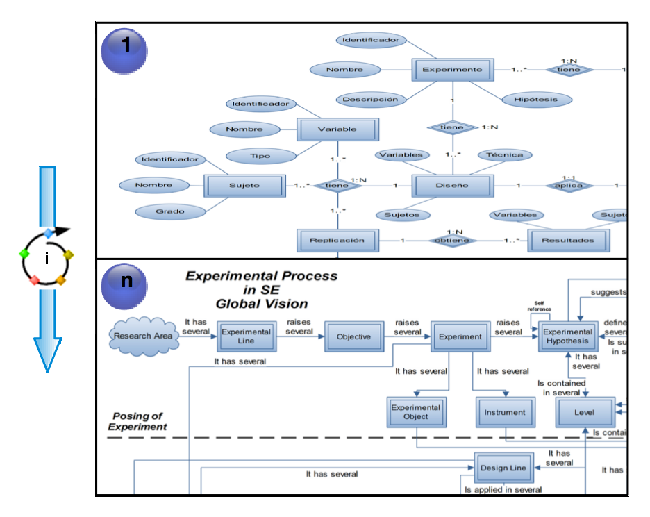
\includegraphics[width=3in]{images/Boseto-Concepts}
	\caption{Extracto del Modelo Conceptual de la Experimentaci�n en GrISE (versi�n final)}
	\label{fig-conceptos-exp-boseto}
\end{figure}

El producto obtenido de este primer proceso de Focus Groups fue un modelo conceptual gen�rico de la experimentaci�n en SE (ver Figura \ref{fig-conceptos-exp-boseto}), el cual no fue consensuado por el grupo. Por lo tanto, se llev� a cabo otro proceso de focus groups, con la particularidad de que cada experimentador indic� �nicamente los conceptos que maneja a trav�s de las actividades que efectivamente realiza en una instancia experimental. Este nuevo ciclo de Focus Groups gener� tres modelos conceptuales, los cuales se muestran en la Figura \ref{fig-conceptos-exp}. Es preciso mencionar que estos modelos responden a los tres roles identificados durante el proceso de entrevistas.

\begin{figure}[htbp!]
	\centering
	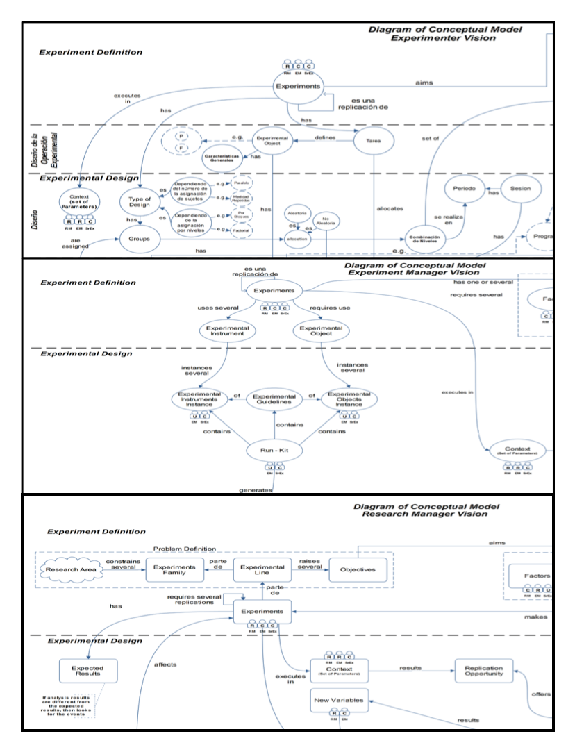
\includegraphics[width=3in]{Images/Concepts}
	\caption{Extracto de los Modelo Conceptuales}
	\label{fig-conceptos-exp}
\end{figure}

Los hallazgos identificados en base a los resultados obtenidos son:

\begin{itemize}
	\item El nivel de detalle conceptual del experimentador que se encarga de la ejecuci�n misma de un experimento es muy alto.
	
	\item Se evidenci� la diversidad terminol�gica entre experimentadores que realizan actividades similares en una instancia experimental en SE.
	
	\item Se evidenci� discrepancia conceptual sobre las actividades de experimentaci�n en SE entre experimentadores.
	
	\item Se confirm� que los conceptos manejados por los experimentadores en SE obedecen a las actividades espec�ficas que realizan en una instancia experimental.
	
	\item Se evidenci� la existencia de roles o perfiles de experimentadores: Experimentadores que custodian el material experimental del grupo, experimentadores que ejecutan en la pr�ctica la experimentaci�n y experimentadores que gestionan con el medio externo los nuevos experimentos y su factibilidad.
\end{itemize}

\subsection{Conclusions Around Software Engineering Experimentation Process}
Los resultados de la investigaci�n constituyen una visi�n expl�cita de la experimentaci�n en SE dentro de un grupo de investigaci�n representativo de la comunidad de ingenier�a de software emp�rica, incluso para los mismos experimentadores que ve�an por primera vez plasmado de forma expl�cita en medios accesibles el modelo de la experimentaci�n en SE. M�s espec�ficamente, las conclusiones obtenidas a partir de esta investigaci�n son:

\begin{enumerate}[(a)]
\item La generalidad de los textos existentes y la diversidad estructural de los reportes experimentales en la comunidad de ingenier�a de software emp�rica no representan una gu�a efectiva para llevar a cabo una instancia experimental en la pr�ctica.
 
\item La falta de formalizaci�n de los reportes experimentales impide realizar una lectura compresiva est�ndar, ya que para cada reporte es preciso descubrir su particularidad al momento de reportar.

\item El uso de formatos distintos en los reportes impide identificar de forma eficiente las actividades llevadas a cabo en una instancia de experimentaci�n en SE.

\item El formato de los archivos que contienen los datos experimentales de las instancias experimentales, no son est�ndar, por lo que es imposible que una persona ajena al grupo de trabajo entienda los conceptos, entidades y acr�nimos utilizados.

\item Se pudo percibir la posibilidad de que la existencia de mecanismos automatizados que guarden el v�nculo entre los experimentos y sus elementos (materiales, raw-data, dise�o, etc.), podr�an ayudar a los experimentadores a no cometer errores, dado el alto n�mero de actividades que deben cubrir.

\item Una comunicaci�n m�s cercana con los experimentadores, permiti� encontrar detalles que generalmente no se reflejan en los reportes experimentales y que ayudaron a entender algunos resultados, conclusiones de los reportes experimentales y llevar a cabo una replicaci�n experimental.

\item Durante las entrevistas personales mantenidas con los experimentadores se evidenci� un tipo de informaci�n impl�cita de los experimentos, la cual no es registrada en ning�n medio. Este tipo de informaci�n posiblemente proviene de la dimensi�n t�cita del conocimiento.

\item La deficiencia en la gesti�n de la informaci�n dentro del GrISE podr�a deberse a la diversidad operativa de los experimentadores, lo que dificulta el intercambio de informaci�n.
\end{enumerate}

\section{The Experimentation in Biotechnology}\label{sec-case-study-2}
La formalidad del proceso experimental de las disciplinas tradicionales nos motiv� a indagar los detalles de las actividades que realizan, para validar la problem�tica identificada en la ESE. La investigaci�n se llev� a acabo en la Universidad de las Fuerzas Armadas ESPE (Ecuador) en la Carrera de Ingenier�a en Biotecnolog�a.

La experimentaci�n en Biotecnolog�a es compleja dado el n�mero de actividades involucradas, la extensa variedad de insumos y los instrumentos que se precisan (dependiendo del �rea de investigaci�n) \cite{Kumar-2014-design-experiment-bioprocessing}. Sin embargo, nuevas propuestas sobre dise�o de experimentos (e.g.: dise�os basados en el enfoque), ofrecen una alternativa de formalizaci�n del proceso experimental \cite{Kumar-2014-design-experiment-bioprocessing}, lo que precisamente fue indagado en la presente investigaci�n.

\subsection{Context}\label{subsec-context-case-study-2}
Para este estudio se consider� a distintos grupos de investigaci�n de la Carrera de Biotecnolog�a. A pesar de que desconocemos el grado de representatividad de los grupos de investigaci�n objeto de estudio, creemos que es alto, dado el nivel de publicaciones realizadas (por citar un par de ejemplos: \cite{Vizuete-2016-green-Synthesis,Villarreal-2016-Effect-Arbuscular,Kumar-2016-In-Vitro-Evaluation}).

De acuerdo al criterio de selecci�n indicado en la Secci�n \ref{sec-methology}, estudiamos las actividades experimentales realizadas por grupos de investigaci�n en las �reas de Biotecnolog�a Humana, Biotecnolog�a Ambiental y Biotecnolog�a Vegetal. Estos grupos est�n liderados por un investigador (generalmente el director de un proyecto o jefe de un laboratorio), e incluyen estudiantes de doctorado y master. Adicionalmente, los grupos mantienen convenios con universidades de distintos pa�ses y disponen de una vasta cantidad de datos experimentales locales y/o p�blicos.

\subsection{Results}\label{subsec-results-case-study-2}
Los resultados obtenidos respecto al estado de la pr�ctica de la experimentaci�n en Biotecnolog�a son descritos en esta secci�n. Las fuentes de informaci�n estudiadas fueron: (1) Literatura referente a los grupos y (2) Conocimiento de los experimentadores.

En este estudio de caso no se realiz� una revisi�n del material experimental existente en los grupos de investigaci�n, dado que era muy espec�fico debido a la naturaleza propia de cada tem�tica de investigaci�n. Es preciso mencionar que los experimentadores indicaron que los datos obtenidos en las instancias experimentales son utilizados hasta su reporte, luego de lo cual son almacenados en repositorios de informaci�n experimental locales o p�blicos para futuros an�lisis. 

\subsubsection{Review of concerning literature}\label{subsubsec-study-literature-case-study-2}
Esta fuente de informaci�n corresponde a textos cient�ficos del �rea de Biotecnolog�a, publicaciones propias de los grupos objeto de estudio y a las denominadas libretas de laboratorio. Dichas fuentes de informaci�n fueron revisadas de forma exhaustiva, lo que permiti� obtener conocimiento y argumentos para generar debates en grupos de discusi�n; as� como, para evaluar y modificar modelos conceptuales y de proceso esbozados en distintas entrevistas. Adem�s, el estudio de las publicaciones de estos grupos permiti� indagar sobre el estado de la pr�ctica de la Biotecnolog�a.

Para realizar el estudio de literatura se utiliz� la t�cnica de an�lisis de documentaci�n (tercer nivel), con el apoyo de software especializado en gesti�n documental, tecnolog�as de la informaci�n, entre otros. Este estudio permiti� abstraer los aspectos fundamentales de la experimentaci�n en Biotecnolog�a, tales como las actividades realizadas y los artefactos utilizados.

The review of the concerning literature obtained the following results:
\begin{itemize}
  \item El proceso de experimentaci�n en Biotecnolog�a est� descrito de forma general en los textos cient�ficos revisados. Por ejemplo en el libro Biotechnology Fundamentals de Khan \cite{Khan-2012-Biotechnology-Fundamentals}.
  
  \item Los textos, gu�as, reportes, etc. sobre experimentaci�n en Biotecnolog�a son numerosos, pero espec�ficos por tem�ticas de investigaci�n. Por ejemplo, en la Biotecnolog�a Agr�cola el libro de Solaiman et al. \cite{Solaiman-2014-Mycorrhizal} describe el uso de microorganismos que se aplican a cultivos para el uso sustentable del suelo. En la Biotecnolog�a Vegetal el libro de Bahadur et al. \cite{Bahadur-2015-Plant-Biotechnology} estudia todas las �micas de \textit{Arabidopsis thaliana} como modelo para el mejoramiento gen�tico de otras plantas.
  
  \item Se encontr� formalidad (terminol�gica y operativa) del proceso de experimentaci�n de Biotecnolog�a en fuentes biogr�ficas de tem�ticas espec�ficas. Por ejemplo, el handbook de Walker et al. \cite{Walker-2008-Handbook-Biomethods} y el libro de Ausubel et al. \cite{Ausubel-2003-Molecular-Biology} denotan mucha similaridad en el protocolo experimental utilizado para el estudio de �cidos nucleicos.
  
  \item Se encontr� diversidad terminol�gica y operativa entre fuentes de distintas tem�ticas. %Por ejemplo en el libro de Villacr�s et al. \cite{Villacres-2015-Banco-HMA} se menciona
  
  \item Los reportes experimentales de los grupos de investigaci�n estudiados son similares en formato y centran su discurso en los resultados generales de cada ensayo (experimento), los cuales se basan en la comparaci�n de  resultados de tratamientos individuales.
  
  \item Encontramos indicios de que las actividades de experimentaci�n realizadas en Biotecnolog�a son el fundamento de la estructura de los reportes experimentales.
  
  \item El estudio de textos cient�ficos permiti� la adquisici�n de un conocimiento general sobre la experimentaci�n en Biotecnolog�a; el cual, en adici�n al conocimiento obtenido de otras fuentes, fue hecho expl�cito en un modelo conceptual b�sico (ver Figura \ref{fig-modelo-conc-inicial}) que sirvi� como insumo inicial en el proceso de grupos de discusi�n.
\end{itemize}

\begin{figure}[htbp!]
	\centering
	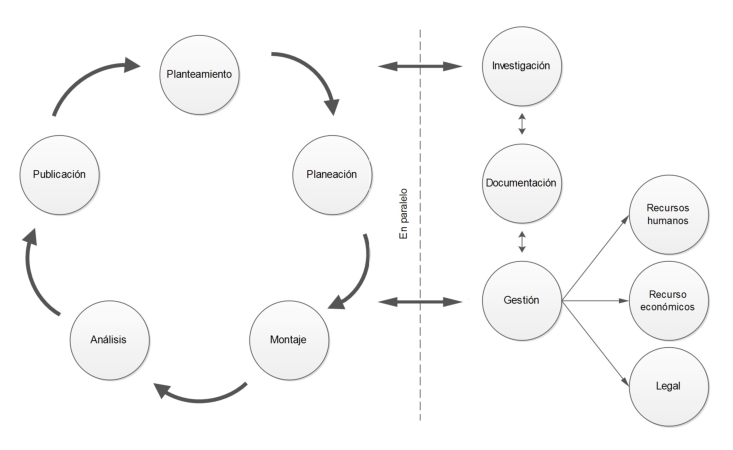
\includegraphics[width=3.2in]{Images/Modelo-Conceptual-Inicial}
	\caption{Modelo Conceptual Inicial}
	\label{fig-modelo-conc-inicial}
\end{figure}

\subsubsection{Obtenci�n de Conocimiento de los Grupos de Investigaci�n}\label{subsubsec-conocimiento-grupos}
El conocimiento obtenido de los grupos de investigaci�n signific� el insumo m�s representativo de esta investigaci�n. Esta actividad permiti� hacer expl�cito el conocimiento de los experimentadores de Biotecnolog�a, lo cual no hab�a sido hecho anteriormente. 

La obtenci�n del conocimiento de los experimentadores se sustent� principalmente en dos t�cnicas: (1) Entrevistas sobre las actividades experimentales que realizan, y (2) Focus Groups sobre los conceptos que manejan.

\textbf{Entrevistas sobre las actividades experimentales de Biotecnolog�a}\\
El proceso de entrevistas a los experimentadores de Biotecnolog�a fue c�clico. Se realizaron varias sesiones con cada experimentador. Por cada sesi�n se gener� un reporte que fue validado por el experimentador en la sesi�n siguiente, hasta llegar a obtener un manuscrito que sintetiza detalladamente las actividades experimentales que lleva a cabo cada experimentador.

De forma paralela a las entrevistas, algunos experimentadores realizaron esbozos en papel o en la pizarra (ver ejemplo en la Figura \ref{fig-proc-exp-esbozo}) sobre las actividades que realizan en el proceso experimental, para poner �nfasis en su relato. Estos esbozos fueron sintetizados en un �nico modelo, el cual fue digitalizado utilizando software especializado. En cada sesi�n fue validado el modelo por los experimentadores (ver Figura \ref{fig-proceso-exp-intermedio}), hasta obtener un modelo final (ver Figura \ref{fig-proceso-exp-final}).

\begin{figure}[htbp!]
	\centering
	\includegraphics[width=3.2in]{Images/Outline-Process}
	\caption{Ejemplo de Esbozo de las Actividades Experimentales de Biotecnolog�a}
	\label{fig-proc-exp-esbozo}
\end{figure}

\begin{figure}[htbp!]
	\centering
	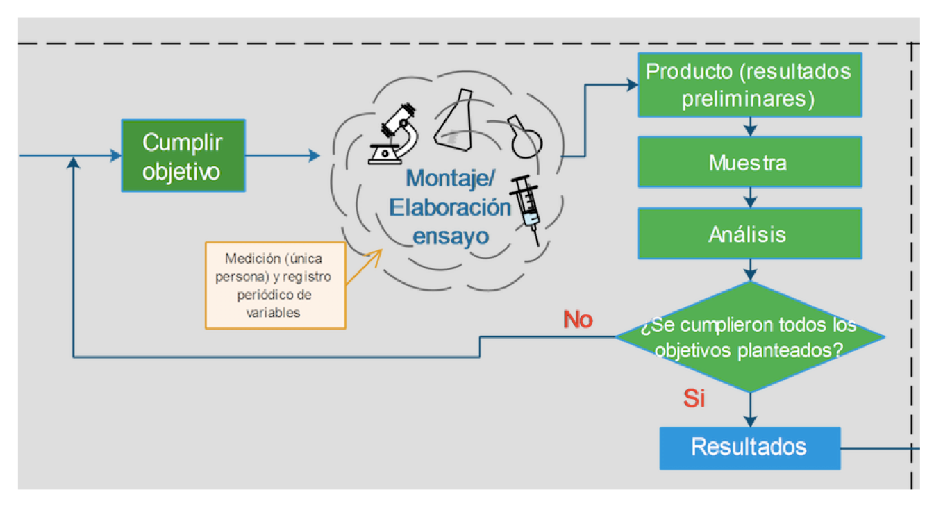
\includegraphics[width=3.2in]{Images/Intermediate-Process}
	\caption{Extracto Inicial del Proceso Experimental de Biotecnolog�a}
	\label{fig-proceso-exp-intermedio}
\end{figure}

\begin{figure}[htbp!]
	\centering
	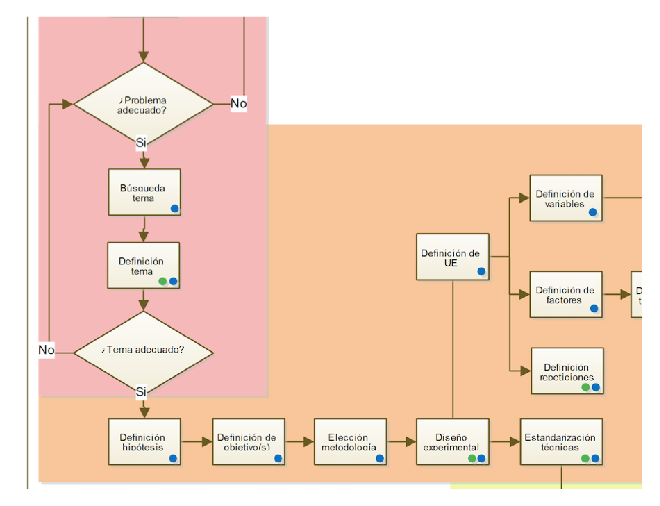
\includegraphics[width=3.2in]{Images/Final-Process}
	\caption{Extracto del Proceso Experimental de Biotecnolog�a}
	\label{fig-proceso-exp-final}
\end{figure}

Como complemento a las entrevistas, se utiliz� t�cnicas de modelado de conceptos, observaci�n participativa y sistemas instrumentales, con el prop�sito de recrear los esbozos de forma fidedigna en herramientas inform�ticas, coadyuvar ideas generadas en la entrevista y recibir feedback complementario a trav�s de medios tecnol�gicos, respectivamente.

Para la aplicaci�n de las t�cnicas mencionadas se utiliz� distintos instrumentos y herramientas, de los cuales destaca la utilizaci�n de mecanismos tecnol�gicos para capturar en video, audio y fotograf�as los detalles de las entrevistas y facilitar su recreaci�n; as� como tambi�n, herramientas inform�ticas para hacer expl�cito el conocimiento adquirido tanto en texto como en gr�ficos.

Los hallazgos obtenidos en torno a la aplicaci�n de las entrevistas son: 

\begin{itemize}
  \item El detalle obtenido en el modelo de procesos sugiere que el protocolo experimental de Biotecnolog�a es formal.
  \item Cada experimentador llevar a cabo actividades espec�ficas dentro del proceso de experimentaci�n en Biotecnolog�a.
  \item El conjunto de actividades realizadas por cada experimentador en Biotecnolog�a tiene una denominaci�n a modo de rol, por ejemplo el \textit{Biometrista} se encarga del an�lisis de datos.
  \item La distribuci�n de actividades experimentales a modo de roles en el proceso de experimentaci�n en Biotecnolog�a, no permite que exista solapamiento de actividades.
\end{itemize}

\textbf{Focus Groups sobre los conceptos manejados en el proceso de experimentaci�n en Biotecnolog�a}\\
El Focus Group para recabar la terminolog�a utilizada en el proceso de experimentaci�n en Biotecnolog�a fue c�clico. El proceso inici� con el debate sobre el modelo conceptual resultante de la review of the concerning literature (ver Figura \ref{fig-modelo-conc-inicial}). A continuaci�n, se realizaron varias sesiones con los experimentadores. De cada sesi�n se obtuvo un producto intermedi� (ver Figura \ref{fig-concepts-draft-bio}), el cual fue validado por el grupo en la siguiente instancia, hasta obtener un producto final (ver Figura \ref{fig-concepts-final-bio}).

\begin{figure}[htbp!]
	\centering
	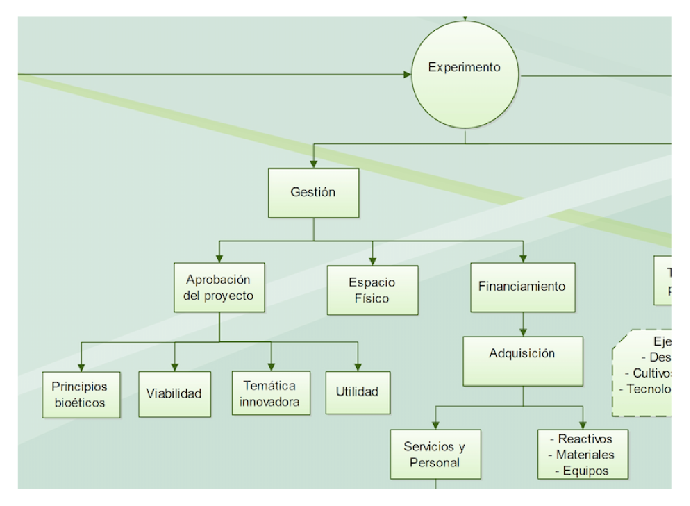
\includegraphics[width=3in]{Images/Concepts-Draft-Bio}
	\caption{Extracto del Modelo Conceptual Inicial de Biotecnolog�a}
	\label{fig-concepts-draft-bio}
\end{figure}

\begin{figure}[htbp!]
	\centering
	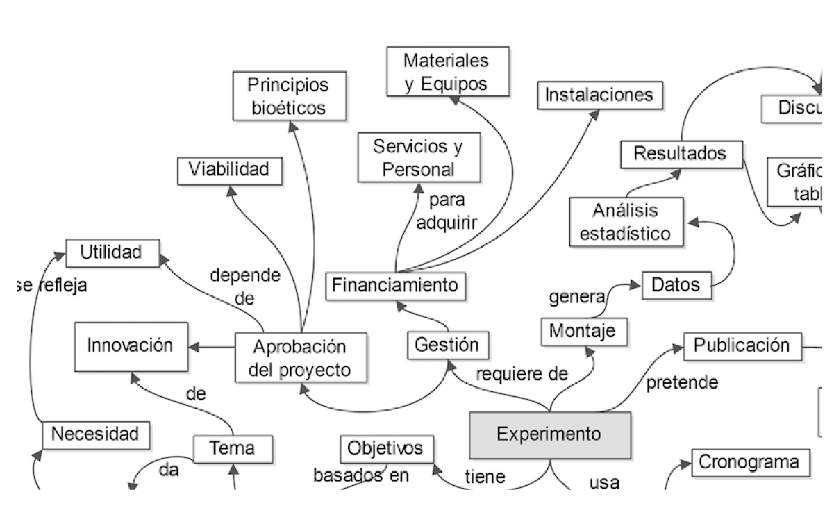
\includegraphics[width=3in]{Images/Concepts-Final-Bio}
	\caption{Extracto del Modelo Conceptual de Biotecnolog�a}
	\label{fig-concepts-final-bio}
\end{figure}

Como complemento al Focus Group se aplicaron t�cnicas de modelado de conceptos, observaci�n participativa y sistemas instrumentales; con el prop�sito de que: los participantes en el focus group puedan esbozar y participar en el modelado conceptual, el investigador participe activamente en el debate sobre las propuestas de los experimentadores y el investigador cubra inquietudes menores con cada experimentador, respectivamente. Con este prop�sito, fueron utilizados los mismos instrumentos y herramientas que en las entrevistas.

Los hallazgos obtenidos en torno al Focus Group son:

\begin{itemize}
	\item La cantidad de conceptos que intervienen en el proceso de experimentaci�n en Biotecnolog�a es alta.
	\item Se constat� que los experimentadores de un mismo grupo de investigaci�n en Biotecnolog�a utilizan una terminolog�a com�n para comunicarse.
	\item Se observ� que los conceptos manejados por los experimentadores en Biotecnolog�a corresponden a las actividades espec�ficas del rol que cumplen en una instancia experimental.
	\item Se constat� no existe duplicaci�n de actividades entre experimentadores en Biotecnolog�a.
\end{itemize}

\subsection{Conclusions}
\begin{enumerate}[(a)]
\item La generalidad de los textos existentes en Biotecnolog�a no representan un gu�a efectiva para llevar a cabo instancias experimentales espec�ficas en la pr�ctica.

\item La formalidad de los reportes experimentales de �reas espec�ficas de la Biotecnolog�a permiten replicar sin mayor complicaci�n los estudios realizados.

\item La formalidad en los reportes permite identificar f�cilmente las actividades llevadas a cabo en una instancia de experimentaci�n.

\item El formato de los contenedores de datos experimentales es est�ndar (hojas excel o repositorios), lo que facilita el acceso y utilizaci�n a otros grupos que investigan sobre la misma tem�tica.

\item El uso de mecanismos automatizados que guarden el v�nculo entre los experimentos y sus elementos (materiales, raw-data, dise�o, etc.) es fundamental y usual en Biotecnolog�a, ya que ayuda a los experimentadores, por ejemplo para gestionar m�s f�cilmente los datos experimentales.

\item Los detalles de los reportes experimentales de Biotecnolog�a son muy claros, tal es as� que sin ser conocedores o peor a�n expertos en el �rea, pudimos entender relativamente bien sus resultados, conclusiones y discuci�n.

\item La efectividad de la gesti�n de la informaci�n dentro de los grupos estudiados podr�a deberse a la formalidad operativa de su proceso; lo que por ende les facilita el intercambio de informaci�n.
\end{enumerate}

\input{tex/comparison}

\section{Survey on Experimentation in Software Engineering}\label{sec-survey}

\section{Discussion and Conclusions}\label{sec-discussion-conclusions}

% Please add the following required packages to your document preamble:
% \usepackage{graphicx}
% \usepackage{lscape}
\begin{landscape}
\begin{table}[]
\centering
\resizebox{\textwidth}{!}{%
\begin{tabular}{llll}
\hline
\# & Hallazgos del estudio en SE & Hallazgos del estudio en biotecnologia & \# \\ \hline
39 & Existe literatura est�ndar, e.g., \textbackslash{}cite\{Wohlin2000,Juristo2001\} &  &  \\
40 & La carencia de literatura est�ndar se suple con reportes o art�culos espec�ficos, e.g., \textbackslash{}cite\{Basili-1986-ESE\} &  &  \\
2 & Se produce diversidad terminol�gica entre fuentes &  &  \\
5 & Existen pocos libros de referencia acerca de experimentaci�n en SE &  &  \\
 &  &  &  \\
 &  &  & 
\end{tabular}%
}
\end{table}
\end{landscape}





%%%%%%%%%%%%%%%%
%%%%%%%%%%%%%%%%
%\begin{table}
%\centering
%\caption{Frequency of Special Characters}
%\begin{tabular}{|c|c|l|} \hline
%Non-English or Math&Frequency&Comments\\ \hline
%\O & 1 in 1,000& For Swedish names\\ \hline
%$\pi$ & 1 in 5& Common in math\\ \hline
%\$ & 4 in 5 & Used in business\\ \hline
%$\Psi^2_1$ & 1 in 40,000& Unexplained usage\\
%\hline\end{tabular}
%\end{table}
%%%%%%%%%%%%%%%%
%%%%%%%%%%%%%%%%



%%%%%%%%%%%%%%%%
%%%%%%%%%%%%%%%%
%\begin{table*}
%\centering
%\caption{Some Typical Commands}
%\begin{tabular}{|c|c|l|} \hline
%Command&A Number&Comments\\ \hline
%\texttt{{\char'134}alignauthor} & 100& Author alignment\\ \hline
%\texttt{{\char'134}numberofauthors}& 200& Author enumeration\\ \hline
%\texttt{{\char'134}table}& 300 & For tables\\ \hline
%\texttt{{\char'134}table*}& 400& For wider tables\\ \hline\end{tabular}
%\end{table*}
% end the environment with {table*}, NOTE not {table}!
%%%%%%%%%%%%%%%%
%%%%%%%%%%%%%%%%



%%%%%%%%%%%%%%%%
%%%%%%%%%%%%%%%%
%\begin{figure}
%\centering
%\includegraphics[height=1in, width=1in]{images/fly}
%\caption{A sample black and white graphic
%that has been resized with the \texttt{includegraphics} command.}
%\end{figure}
%%%%%%%%%%%%%%%%
%%%%%%%%%%%%%%%%


%%%%%%%%%%%%%%%%
%%%%%%%%%%%%%%%%
%\begin{figure*}
%\centering
%\includegraphics{images/flies}
%\caption{A sample black and white graphic
%that needs to span two columns of text.}
%\end{figure*}
%%%%%%%%%%%%%%%%
%%%%%%%%%%%%%%%%

%%%%%%%%%%%%%%%%
%%%%%%%%%%%%%%%%
%\begin{figure}
%\centering
%\includegraphics[height=1in, width=1in]{images/rosette}
%\caption{A sample black and white graphic that has
%been resized with the \texttt{includegraphics} command.}
%\vskip -6pt
%\end{figure}
%%%%%%%%%%%%%%%%
%%%%%%%%%%%%%%%%
%\
%ACKNOWLEDGMENTS are optional
\section{Acknowledgments}
This section is optional; it is a location for you
to acknowledge grants, funding, editing assistance and
what have you.  In the present case, for example, the
authors would like to thank Gerald Murray of ACM for
his help in codifying this \textit{Author's Guide}
and the \textbf{.cls} and \textbf{.tex} files that it describes.

%
% The following two commands are all you need in the
% initial runs of your .tex file to
% produce the bibliography for the citations in your paper.
\bibliographystyle{abbrv}
\bibliography{Bibliografia}  % sigproc.bib is the name of the Bibliography in this case
% You must have a proper ".bib" file
%  and remember to run:
% latex bibtex latex latex
% to resolve all references
%
% ACM needs 'a single self-contained file'!
%
%APPENDICES are optional
%\balancecolumns
%\appendix
%Appendix A
%\section{Headings in Appendices}
%The rules about hierarchical headings discussed above for
%the body of the article are different in the appendices.
%In the \textbf{appendix} environment, the command
%\textbf{section} is used to
%indicate the start of each Appendix, with alphabetic order
%designation (i.e. the first is A, the second B, etc.) and
%a title (if you include one).  So, if you need
%hierarchical structure
%\textit{within} an Appendix, start with \textbf{subsection} as the
%highest level. Here is an outline of the body of this
%document in Appendix-appropriate form:
%\subsection{Introduction}
%\subsection{The Body of the Paper}
%\subsubsection{Type Changes and  Special Characters}
%\subsubsection{Math Equations}
%\paragraph{Inline (In-text) Equations}
%\paragraph{Display Equations}
%\subsubsection{Citations}
%\subsubsection{Tables}
%\subsubsection{Figures}
%\subsubsection{Theorem-like Constructs}
%\subsubsection*{A Caveat for the \TeX\ Expert}
%\subsection{Conclusions}
%\subsection{Acknowledgments}
%\subsection{Additional Authors}
%This section is inserted by \LaTeX; you do not insert it.
%You just add the names and information in the
%\texttt{{\char'134}additionalauthors} command at the start
%of the document.
%\subsection{References}
%Generated by bibtex from your ~.bib file.  Run latex,
%then bibtex, then latex twice (to resolve references)
%to create the ~.bbl file.  Insert that ~.bbl file into
%the .tex source file and comment out
%the command \texttt{{\char'134}thebibliography}.
% This next section command marks the start of
% Appendix B, and does not continue the present hierarchy
%\section{More Help for the Hardy}
%The sig-alternate.cls file itself is chock-full of succinct
%and helpful comments.  If you consider yourself a moderately
%experienced to expert user of \LaTeX, you may find reading
%it useful but please remember not to change it.
%\balancecolumns % GM June 2007
% That's all folks!
\end{document}
